\documentclass[a4paper,12pt]{article} % добавить leqno в [] для нумерации слева
\usepackage[a4paper,top=1.3cm,bottom=2cm,left=1.5cm,right=1.5cm,marginparwidth=0.75cm]{geometry}
%%% Работа с русским языком
\usepackage{cmap}					% поиск в PDF
\usepackage[warn]{mathtext} 		% русские буквы в фомулах
\usepackage[T2A]{fontenc}			% кодировка
\usepackage[utf8]{inputenc}			% кодировка исходного текста
\usepackage[english,russian]{babel}	% локализация и переносы
\usepackage{multirow}
\usepackage{float}
\restylefloat{table}


%\graphicspath{ {images/}}
\usepackage{graphicx}

\usepackage{wrapfig}
\usepackage{tabularx}

\usepackage{hyperref}
\usepackage[rgb]{xcolor}
\hypersetup{
	colorlinks=true,urlcolor=blue
}

%%% Дополнительная работа с математикой
\usepackage{amsmath,amsfonts,amssymb,amsthm,mathtools} % AMS
\usepackage{icomma} % "Умная" запятая: $0,2$ --- число, $0, 2$ --- перечисление

%% Номера формул
\mathtoolsset{showonlyrefs=true} % Показывать номера только у тех формул, на которые есть \eqref{} в тексте.

%% Шрифты
\usepackage{euscript}	 % Шрифт Евклид
\usepackage{mathrsfs} % Красивый матшрифт

%% Свои команды
\DeclareMathOperator{\sgn}{\mathop{sgn}}

%% Перенос знаков в формулах (по Львовскому)
\newcommand*{\hm}[1]{#1\nobreak\discretionary{}
	{\hbox{$\mathsurround=0pt #1$}}{}}

\date{\today}

\title{Лабораторная работа 1.2.2 Экспериментальная проверка закона вращательного движения на крестообразном маятнике}
\date{}
\begin{document}
\maketitle
\section{Аннотация}
\subsection{Цель работы}
Экспериментально проверить уравнение \eqref{1}, получив зависимость углового ускорения от момента инерции и момента
прикладываемых к системе сил, а также проанализировать влияние
сил трения, действующих в оси вращения.

\subsection{Используемые приборы}
В работе используется крестообразный «маятник» (рис. \ref{pic}), перегрузки разной массы, установка с датчикам и компьютер, с помощью которого происходит управление.

\subsection{Ожидаемые результаты}
Убедимся в справедливости соотношения \eqref{1}, на основе экспериментальных данных получим зависимость углового ускорения от момента инерции и момента прикладываемых к системе сил. Проанализируем влияние на результаты сил трения в оси.

\section{Теоретические сведения}
Закон вращательного движения:
\begin{gather}
	\hat{I}\ddot{\varphi} =\overset{\to}{ M} \label{1},\text{ где } \ddot{\varphi} \equiv \dot{\omega} \equiv \vec\beta, \ \overset{\to}{ M} = \sum_i \overset{ \to}{ M_i}
\end{gather}
\begin{figure}[h!]
\begin{center}
    \label{pic}
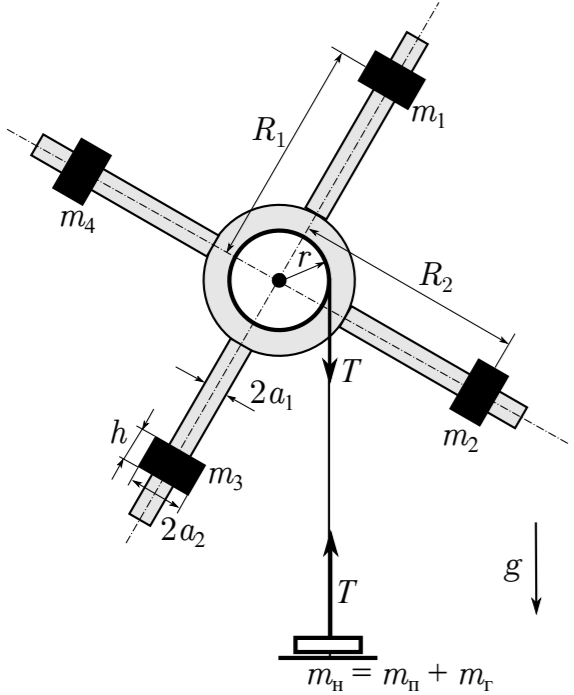
\includegraphics[width=0.5\textwidth]{images/Маятник.png}
\end{center}
\caption{Крестообразный маятник Обербека} \label{маятник}
\end{figure}
На маятник действуют два момента сил: силы натяжения нити $M_T: M_T = rT$, где $r$ - радиус шкива и момент силы трения $ M_\text{тр} $ 
Силу$ T $ выразим из уравнения движения платформы:\begin{gather}
	(m_\text{п} + m_\text{г})\beta r = (m_\text{п} + m_\text{г})g - T \implies M_T =(m_\text{п} + m_\text{г})r(g - \beta r),
\end{gather} где $ m_\text{п} $ -- масса платформы,$ m_\text{г} $ -- масса грузика. 
Пусть $ m_H = (m_\text{п} + m_\text{г}) $ 
Откуда согласно основному уравнению вращательного движения :
\begin{equation}
(I+m_Hr^2)\beta = m_Hgr-M_\text{тр}
\label{M_T}
\end{equation}

Рассмотрим момент силы трения. Его зависимость от скорости не ясна, однако может иметь как составляющую, пропорциональную силе реакции в оси $N$ (сухое трение), так и составляющую, пропорциональную угловой скорости вращения (вязкое трение). Учитывая, что сила реакции уравновешенного маятника равна $ N = m_\text{м}g + T \approx (m_\text{м} + m_\text{н})g \approx m_\text{м}g $,  где$ m_\text{м} $ -- масса маятника. Тогда:
\begin{equation}
M_\text{тр} \simeq \left(1 + \frac{m_H}{m_M}\right) M_0 + \eta \omega \approx M_0 +\eta \omega
\label{трение}
\end{equation} 
где $M_0$ - момент сил трения для покоящегося маятника при нулевой массе подвеса, $m_M$ - масса маятника 

Для расчета момента инерции системы, предположим, что грузы $m_i$ имеют форму полых цилиндров, внутренний и внешний радиус которых известен, образующая h
\begin{equation}
I = I_0 + \sum_{i=1}^4(I_i+m_iR_i^2)
\label{I}
\end{equation}
где $I_0$ - момент инерции системы без грузов, $R_i$ -  расстояние от центров масс грузов до оси вращения
\begin{equation}
I_i = \frac{1}{12}m_ih^2+\frac{1}{4}m_i(a_1^2+a_2^2)
\label{Ii}
\end{equation} -- момент инерции груза относительно оси, проходящей через его центр масс.

\textbf{Используемые приближения:} 
\begin{gather}
	m_\text{м} \gg m_\text{н} \\ 
	m_\text{н} r^2 \ll I \implies M_\text{н} \approx m_\text{н}gr \implies T \approx m_\text{н}g
\end{gather} 
\newpage
\section{Методика измерений}
В работе предлагается провести следующие измерения
\begin{enumerate}
	\item  Исследовать вращательное движение маятника под действием
	различных перегрузков при постоянном моменте инерции системы $ I $ (положения $ R_i $ грузов фиксированы).
	Результатом будет зависимость начального углового ускорения $ \beta_0 $ от массы нагрузки $ m_ \text{н} $ , откуда  может быть определён момент инерции системы 
	и минимальный момент силы трения.
	\item Затем предлагается изучить вращательное движение маятника при различных значениях момента инерции системы (фиксирована
	масса $ m_ \text{н} $. Момент инерции можно варьировать, изменяя расстояния $ R_i $ центров масс грузов от оси вращения. Измеренные значения
	 $ I $ сравниваются с расчетными.
\end{enumerate}
\textbf{Балансировка маятника} Для проверки зависимостей необходимо, чтобы маятник был уравновешен -- то есть его центр масс
оси вращения. Несбалансированность приводит к следующим эффектам: во-первых, появляется
зависимость момента силы тяжести от угла поворота маятника; во-вторых, возникают дополнительные пульсации силы реакции $ N $ из-за центростремительного ускорения центра масс)
и, следовательно, момента силы трения в подшипниках $ M_ \text{тр} $ .Оба
фактора могут привести к существенному отклонению от линейной зависимости измеряемой функции $ \beta(\omega) $.
\section{Используемое оборудование}
В работе используется крестообразный маятник, состоит из четырех тонкий стержней, перпендикулярных друг другу, укрепленных на втулке. Втулка и два шкива насажены на общую ось, вся система благодаря подшипникам может вращаться вокруг горизонтальной оси. Установка позволяет автоматически фиксировать моменты прохождения концов стержня через датчик.

\textbf{Погрешности:}\newline
Погрешность измерений определяются по компьютеру. Погрешность штангенциркуля $ 0.5 $~мм.
\section{Результаты измерений и обработка данных}
\begin{table}[!ht]
    \centering
    \begin{tabular}{|c|c|c|c|}
    \hline
        $\beta_0, c^{-2}$ & $\Delta \beta, c^{-2}$ & $k, c^{-1}$ & $\Delta k, c^{-1}$ \\ \hline
        0,337 & 0,0056 & -0,009 & 0,0053 \\ \hline
        0,3779 & 0,0052 & -0,0014 & 0,0048 \\ \hline
        0,3533 & 0,0064 & -0,01057 & 0,0061 \\ \hline
        0,3561 & 0,0057 & -0,0070 & 0,0054  \\ \hline
    \end{tabular}
    \caption{$\beta_0(\omega)$ при $m=42.5$~г}
\end{table}
\begin{table}[!ht]
    \centering
    \begin{tabular}{|c|c|c|c|}
    \hline
        $\beta_0, c^{-2}$ & $\Delta \beta, c^{-2} $& $k, c^{-1}$ & $\Delta k, c^{-1}$ \\ \hline
        0,8008 & 0,0056 & -0,01442 & 0,0035  \\ \hline
        0,7984 & 0,0024 & -0,0141 & 0,0015  \\ \hline
        0,777 & 0,0027 & -0,01359 & 0,0017  \\ \hline
        0,7921 & 0,0036 & -0,0140 & 0,0022  \\ \hline
    \end{tabular}
    \caption{$\beta_0(\omega)$ при $m=79.0$~г}
\end{table}
\begin{table}[!ht]
    \centering
    \begin{tabular}{|c|c|c|c|}
    \hline
        $\beta_0, c^{-2}$ & $\Delta \beta, c^{-2}$ & $k, c^{-1}$ & $\Delta k, c^{-1}$ \\ \hline
        1,162 & 0,0051 & -0,01976 & 0,0026  \\ \hline
        1,144 & 0,0023 & -0,02033 & 0,0027  \\ \hline
        1,133 & 0,0025 & -0,01943 & 0,0023  \\ \hline
        1,1463 & 0,0033 & -0,0198 & 0,0025  \\ \hline
    \end{tabular}
    \caption{$\beta_0(\omega)$ при $m=106.1$~г}
\end{table}
\begin{table}[!ht]
    \centering
    \begin{tabular}{|c|c|c|c|}
    \hline
        $\beta_0, c^{-2}$ & $\Delta \beta, c^{-2}$ &$ k, c^{-1}$ & $\Delta k, c^{-1}$ \\ \hline
        1,561 & 0,0035 & -0,009 & 0,0015  \\ \hline
        1,524 & 0,0029 & -0,0014 & 0,0015  \\ \hline
        1,572 & 0,003 & -0,01057 & 0,0021  \\ \hline
        1,5523 & 0,0031 & -0,0070 & 0,0017  \\ \hline
    \end{tabular}
    \caption{$\beta_0(\omega)$ при $m=143.2$~г}
\end{table}
\begin{table}[!ht]
    \centering
    \begin{tabular}{|c|c|c|c|}
    \hline
        $\beta_0, c^{-2}$ & $\Delta \beta, c^{-2}$ & $k, c^{-1}$ & $\Delta k, c^{-1}$ \\ \hline
        1,996 & 0,0028 & -0,01998 & 0,0011  \\ \hline
        2,034 & 0,0025 & -0,02001 & 0,0014  \\ \hline
        1,988 & 0,0029 & -0,01989 & 0,0016  \\ \hline
        2,0060 & 0,0027 & -0,0200 & 0,0014  \\ \hline
    \end{tabular}
    \caption{$\beta_0(\omega)$ при $m=179$~г}
\end{table}
\begin{table}[!ht]
    \centering
    \begin{tabular}{|c|c|c|c|}
    \hline
        $\beta_0, c^{-2}$ & $\Delta \beta, c^{-2}$ & $k, c^{-1}$ & $\Delta k, c^{-1}$ \\ \hline
        0,9753 & 0,0031 & -0,01281 & 0,0017  \\ \hline
        0,9602 & 0,0059 & -0,01191 & 0,0033  \\ \hline
        0,9698 & 0,0035 & -0,01235 & 0,0026  \\ \hline
        0,9684 & 0,0042 & -0,0124 & 0,0025  \\ \hline
    \end{tabular}
    \caption{$\beta_0(\omega)$ при $m=143.2$~г и $R= 10,4$~см}
\end{table}
\begin{table}[!ht]
    \centering
    \begin{tabular}{|c|c|c|c|}
    \hline
        $\beta_0, c^{-2}$ & $\Delta \beta, c^{-2}$ & $k, c^{-1}$ & $\Delta k, c^{-1}$ \\ \hline
        0,8033 & 0,0036 & -0,01149 & 0,0036  \\ \hline
        0,8145 & 0,0024 & -0,01163 & 0,0032  \\ \hline
        0,8067 & 0,0033 & -0,01139 & 0,0029  \\ \hline
        0,8082 & 0,0031 & -0,0115 & 0,0032  \\ \hline
    \end{tabular}
    \caption{$\beta_0(\omega)$ при $m=143.2$~г и $R= 15,9$~см}
\end{table}
\begin{table}[!ht]
    \centering
    \begin{tabular}{|c|c|c|c|}
    \hline
        $\beta_0, c^{-2}$ & $\Delta \beta, c^{-2}$ & $k, c^{-1}$ & $\Delta k, c^{-1}$ \\ \hline
        0,6451 & 0,0028 & -0,0105 & 0,0018  \\ \hline
        0,6634 & 0,0024 & -0,0097 & 0,0021  \\ \hline
        0,6311 & 0,0031 & -0,0111 & 0,0023  \\ \hline
        0,6465 & 0,0028 & -0,0104 & 0,0021  \\ \hline
    \end{tabular}
    \caption{$\beta_0(\omega)$ при $m=143.2$~г и $R= 17,1$~см}
\end{table}
\begin{table}[H]
    \centering
    \begin{tabular}{|c|c|c|c|}
    \hline
        $\beta_0, c^{-2}$ & $\Delta \beta, c^{-2}$ & $k, c^{-1}$ & $\Delta k, c^{-1}$ \\ \hline
        0,8683 & 0,0059 & -0,02252 & 0,0035  \\ \hline
        0,9214 & 0,0067 & -0,02882 & 0,0043  \\ \hline
        ~ & ~ & ~ &   \\ \hline
        0,89485 & 0,0063 & -0,02567 & 0,0039  \\ \hline
    \end{tabular}
    \caption{$\beta_0(\omega)$ пустой установки}
\end{table}
\newpage
При проведении эксперимента пустая платформа приходила в движение, когда дополнительная масса равнялась $ m =  6.7 ~ \text{г}$  \begin{gather}
    M_0 = (m_{ \text{платформы}}+ m)gr = 2.01\pm_0.01 ~\text{мН} \cdot \text{м}^2  
\end{gather}  
Построим график $ \beta_0\left(M_{\text{трения}}\right) $:
\begin{figure}[h!]
    \centering
    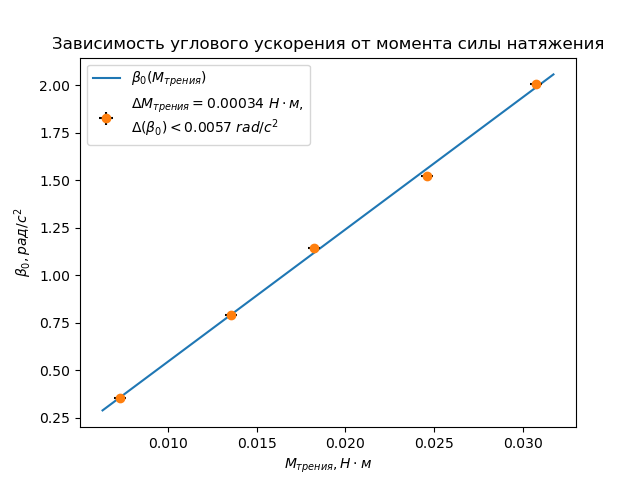
\includegraphics[width=0.8\textwidth]{images/a.png}
\end{figure}
\newline
По графику определим коэффициент наклона $ k \approx 69.59~ \text{рад}/(\text{Н}\cdot \text{м} \cdot \text{с}^{2}), b = 0,1499 ~ \text{рад}/ \text{с}^2 $. Тогда \begin{gather}
    I = \frac{1}{k} \approx 14,37 ~ \text{г} \cdot \text{м}^2 \\
    M_0 = - b \cdot I \approx 2,15 ~ \text{мН} \cdot \text{м}^2 \\
    \varepsilon_{I} \approx 0,023 \% \\
    I = 14,37 \pm 0,32 \text{г} \cdot \text{м}^2 \\
    \varepsilon_{M_0} = \varepsilon_I + \varepsilon_{\beta_0} \implies \Delta M_0 = 0,06~  \text{мН} \cdot \text{м}^2 \implies M_0 = 2,15 \pm 0,06~  \text{мН} \cdot \text{м}^2
\end{gather}
Построим график $ I(R^2) $: \newline
\begin{figure}[h!]
    \centering
    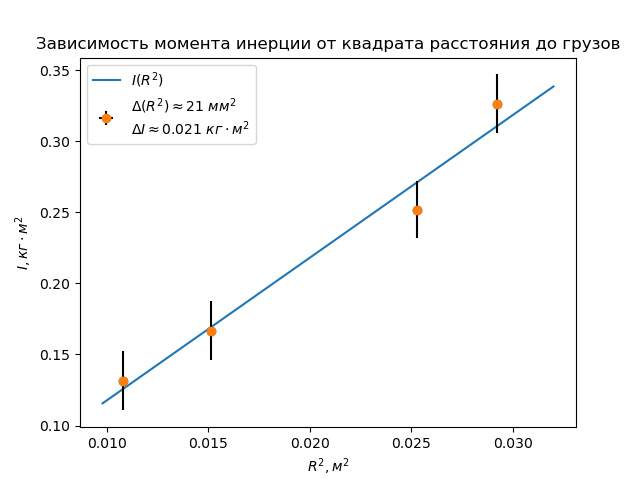
\includegraphics[width=0.8\textwidth]{images/b.png}
\end{figure}

Получили значение из графика $ b = 17,1 ~ \text{г} \cdot \text{м}^2  $. 
По формуле \eqref{I} вычислим слагаемое $ \sum_{i=1}^4(I_i\hm{+}m_iR_i^2) $. Поскольку $ \forall i, j \in: \{1, 2, 3, 4\}\ R_i \approx R_j $, поэтому $ \sum_{i=1}^4(I_i\hm{+}m_iR_i^2) \approx 4I_1 $. 
 \begin{gather}
    \frac{1}{12} m_1 h^2 + \frac{1}{4} m_1 (a_1^2 + a_2^2) \approx 7,5 \cdot\,10^{ - 5} \ll b \implies I_0 \approx b = 17,1~\text{г} \cdot \text{м}^2 \\
    \varepsilon_{I_0} = \Delta I \approx 0,021~ \text{г} \cdot \text{м}^2 \implies I_0 = 17,1\pm 0,021~\text{г} \cdot \text{м}^2\, 
\end{gather}
По формуле $I_0 = \dfrac{m_ \text{п}gr  - M_0}{\beta_0} $: \begin{gather}
    I_0 = 17,71 \pm 0,35 ~\text{г} \cdot \text{м}^2
\end{gather}  
\section{Обсуждение результатов}
В эксперименте были получены неточные результаты(так, значения $ I_0 $ и $ M_0 $ не совпадают по двум различным способам их измерения). Мы пришли к неверным результатам, поскольку
наш маятник не был хорошо сбалансирован. Из-за этого у системы появился дополнительный момент сил, о котором мы можем
понять по тому, что значения для $ I_0 $ и $ M_0 $, которые получены без использования углового ускорения, которое меняется из-за разбалансировки, больше, чем те, которые использовали зависимость с угловым ускорением.
В качестве решения такого вида разбалансировки предлагается ввести эффективный момент инерции пустой установки $ I^\ast = I_0 + I $. Тогда, не меняя расположение грузов, мы сможем учесть нескомпенсированный момент сил и получить результаты 
соответствующие ожидаемым по точности. В качестве альтернативы предлагается использовать опыт и способности других студентов, которые смогли хорошо сбалансировать маятник и не разбалансировать его в процессе работы.

Стоит отметить, что разбалансировка, которая была у нашего маятника, была незначительна на тех, границах диапазона моментов сил, на котором проводились эксперименты, и, кроме того имела постоянный характер воздействия,
поэтому на полученных графиках мы можем построить прямую в пределах рассчитанных погрешностей и подтвердить характер зависимостей, которые хотели доказать.
\section{Вывод}
\begin{enumerate}
    \item Мы попытались ввести маятник в безразличное положение равновесие, однако, в силу неаккуратности, не смогли 
    зафиксировать маятник в сбалансированном состоянии. Мы выбрали положение, которое на наш взгляд было наиболее близко к положению безразличного равновесия
    , которое мы намеревались достигнуть, и записали значения $ R_i $/
    \item Оценили момент силы трения в подшипниках. Для этого мы выбирали грузы различных масс и нашли такой, начиная с которого платформа начинает опускаться. Таким образом нашли $ M_0 $ первым способом.
    \item Познакомились с расчетно-измерительной системой Kinematic, научились делать измерения и получать выходные данные с помощью неё
    \item Измерили для одного и того же положения грузов угловое ускорение для грузов различных масс в диапазоне от 20г до 200г, построили график $ \beta(M_{ \text{трения}}) $, и получили $ M_0 $ вторым способом и момент инерции установки $ I $ . $ M_0 $ измеренные разными способами не 
    совпадают в пределах погрешностей, однако отличаются лишь на $ 6,5\% $. 
    \item Измерили угловые ускорения для одного и того же груза, но разных положений грузов на маятнике. Используя результаты предыдущего пункта посчитали моменты инерции и построили график $ I(R^2) $. По нему определили момент инерции пустой установки $ I_0 $ первым способом.
    \item Измерили угловое ускорение ускорение пустой установки  вторым способом. Данные значения также не совпали в пределах погрешностей, но отличаются незначительно -- $ 3,4\% $.
    \item Поразмышляли о том, почему мы получили такие результаты.
\end{enumerate}
\end{document}